\documentclass[11pt, xcolor = {dvipsnames}]{beamer}
\usepackage[spanish]{babel}
\usepackage[utf8]{inputenc}
\usepackage{tikz}
\usepackage{hyperref}
\usetikzlibrary{trees, matrix, positioning, external}
% \tikzexternalize[prefix = Figures/]


\tikzset{
  tree/.style = {
    level distance = 5cm,
    sibling distance = 7cm,
    ->,
    ultra thick,
    ampersand replacement = \&
  },
  board/.style = {
    matrix of nodes,
    row sep = -\pgflinewidth,
    column sep = -\pgflinewidth,
    -,
    nodes = {rectangle, draw = black, fill = blue!20, align = center},
    ultra thick,
    font = \huge\bf,
    minimum size = 1.1cm,
    % nodes in empty cells,
    ampersand replacement = \&
  },
  marker/.style = {
    opacity = .4,
    -,
    line width = 7mm,
    line cap = round,
    color = #1
  },
  cross/.style = {
    -,
    line width = 4mm,
    color = red
  },
  fig/.style = {
    circle,
    draw = black!70,
    very thick
  },
  line/.style = {
    ->,
    very thick
  }
}


\newcommand{\x}{\color{OliveGreen}{X}}
\renewcommand{\o}{\color{RoyalBlue}{O}}
\newcommand{\e}{\color{blue!20}{X}}
\newcommand{\EB}{child { node {\scalebox{2}{Estrategia básica}}}}
\newcommand{\cross}[1]{
  \draw[cross] (#1-1-1.north west) to (#1-3-3.south east);
  \draw[cross] (#1-3-1.south west) to (#1-1-3.north east);
}


\usetheme{Rochester}


\title{Tres en raya con \textit{Raspberry Pi}}
\subtitle{Proyecto II}
\author{David Álvarez \and Guillermo Creus}
\institute[ETSEIB]{
  Escuela Técnica Superior de Ingeniería Industrial de Barcelona \\
  Universidad Politécnica de Cataluña
}
\date{\today}
\titlegraphic{
  
\includegraphics[height = 1.5cm]{Logo_ETSEIB.png}
  \hspace{1cm}
  
\includegraphics[height = 1.5cm]{Logo_UPC.png}
}



\begin{document}

\frame{\titlepage}


\section{Introducción}

\begin{frame}{Visión general del proyecto}
  \begin{figure}
    \centering
    \begin{tikzpicture}
      \node[fig] (ord) {
\includegraphics[width=2 cm]{ordenador.png}};
      \node[fig, right = 4cm of ord] (brazo) {
\includegraphics[width=2 cm]{brazo_robotico.png}};
      \node[fig, below right = .75cm and .75cm of ord] (rasp)  {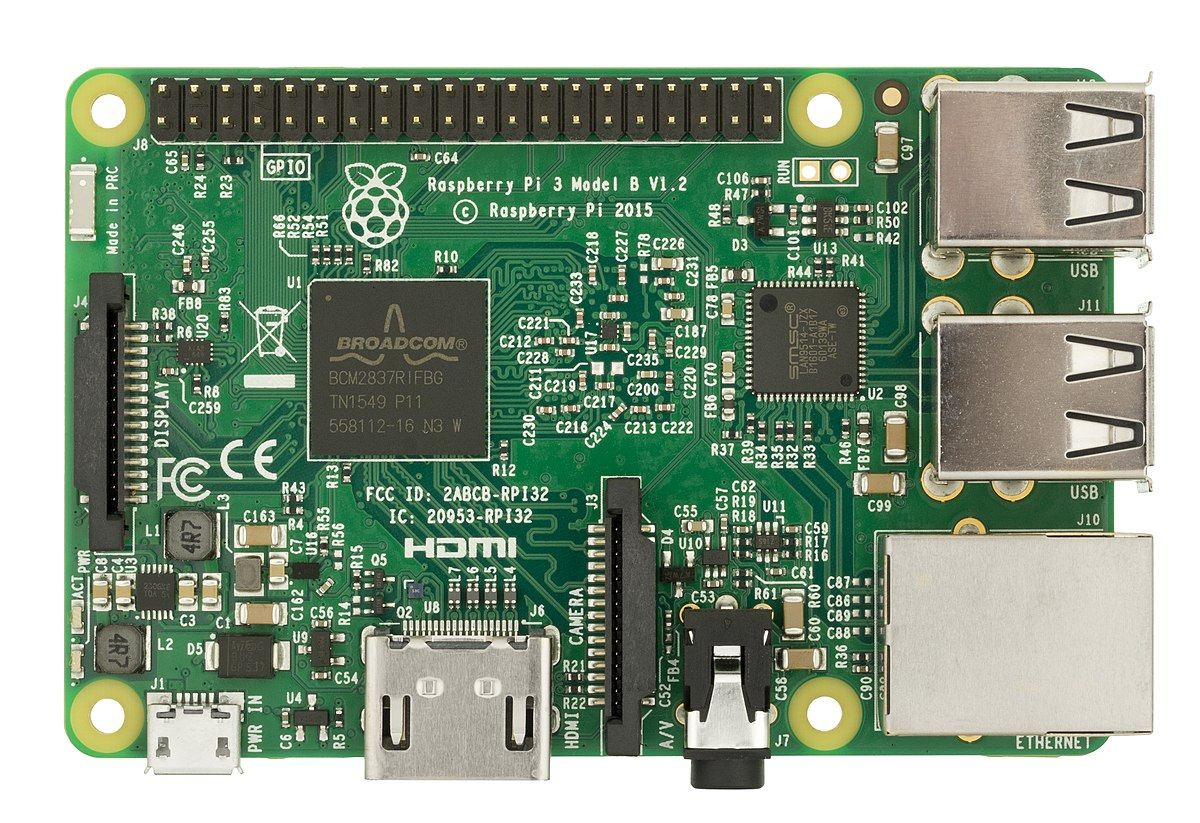
\includegraphics[width=3 cm]{raspberry.jpeg}};
      \draw[line] (ord.north east) to [bend left = 20] (brazo.north west);
      \draw[line] (brazo.west) to (ord.east);
      \draw[line] (ord.south) to [bend right = 20] (rasp.west);
      \draw[line] (rasp) to (ord);
      \draw[line] (rasp.east) to [bend right = 20] (brazo.south);
      \draw[line] (brazo) to (rasp);
    \end{tikzpicture}
  \end{figure}
  \note{
    David, si puedes de este diagrama saca la flecha que va del robot a a la Raspberry, y las flechas que van del robot al ordenador/móvil pq en realidad por ahí no circula información (como veas).\\ \\

    Sería interesar comentar que tipo de servidor utilizamos y el tema IP local.
  }
\end{frame}


\section{Tres en raya}
\begin{frame}{Funcionamiento programa 3 en raya}
  \begin{itemize}
    \item Provee una respuesta al input proporcionado
    \item Juego suma cero $\Rightarrow$ con una estrategia correcta se puede evitar perder
    \item Desarrollo del árbol de posibilidades, evitando las ramas perdedoras
    \item \textbf{FINALIDAD:} Dado un tablero, "guiar"  la partida hacia una posición ganadora o acabar en tablas mediante una \textit{estrategia básica.}
  \end{itemize}
\end{frame}

\begin{frame}{Descarte de tableros según simetrías}
  \begin{columns}
    \column{0.5\textwidth}
    \begin{figure}
      \centering
      \scalebox{.5}{
        \begin{tikzpicture}
          \node[board, draw] (R) {
            \x \& \e \& \e \\
            \e \& \e \& \e \\
            \e \& \e \& \e \\
          };
          \node[board, right = of R] (A) {
            \x \& \o \& \e \\
            \e \& \e \& \e \\
            \e \& \e \& \e \\
          };
          \node[board, right = of A] (B) {
            \x \& \e \& \o \\
            \e \& \e \& \e \\
            \e \& \e \& \e \\
          };
          \node[board, below = of R] (C) {
            \x \& \e \& \e \\
            \o \& \e \& \e \\
            \e \& \e \& \e \\
          };
          \node[board, below = of A] (D) {
            \x \& \e \& \e \\
            \e \& \o \& \e \\
            \e \& \e \& \e \\
          };
          \node[board, below = of B] (E) {
            \x \& \e \& \e \\
            \e \& \e \& \o \\
            \e \& \e \& \e \\
          };
          \node[board, below = of C] (F) {
            \x \& \e \& \e \\
            \e \& \e \& \e \\
            \o \& \e \& \e \\
          };
          \node[board, below = of D] (G) {
            \x \& \e \& \e \\
            \e \& \e \& \e \\
            \e \& \o \& \e \\
          };
          \node[board, below = of E] (H) {
            \x \& \e \& \e \\
            \e \& \e \& \e \\
            \e \& \e \& \o \\
          };
          \pause
          \draw[<->, ultra thick] (A-3-1.south west) to node[right]{Simetría}
          (C-1-3.north east);
          \draw[<->, ultra thick] (B-3-1.south west) to node[right, very near
          start]{Simetría} (F-1-3.north east);
          \draw[<->, ultra thick] (E-3-1.south west) to node[right]{Simetría}
          (G-1-3.north east);
          \pause
          \cross{C}
          \cross{F}
          \cross{G}
        \end{tikzpicture}
      }
    \end{figure}
    \column{0.3\textwidth}
    \begin{itemize}
      \item Permite pasar de $9!$ (362800) tableros a 30.
    \end{itemize}
    \note<3>{
      Yo pasaría directamente a la diapositiva con las cruces rojas para aligerar la presentación (pero no sé sacar la diapositiva intermedia)
    }
  \end{columns}
\end{frame}

\section{Servidor}
\begin{frame}{Estrategia básica}
  \begin{columns}
    \column{0.6\textwidth}
    \begin{figure}
      \centering
      \scalebox{.5}{
        \begin{tikzpicture}[tree]
          \node[board] (20) {
            \o \& \e \& \e \\
            \o \& \e \& \x \\
            \e \& \e \& \x \\
          }
          child {
            node[board] (21) {
              \o \& \e \& \e \\
              \o \& \e \& \x \\
              \x \& \e \& \x \\
            }
          }
          child {
            node[board] (22) {
              \o \& \e \& \x \\
              \o \& \e \& \x \\
              \e \& \e \& \x \\
            }
          };
          % \draw[marker = RoyalBlue] (1-1-1.north west) to (1-3-3.south east);
          \draw[marker = OliveGreen] (22-3-3.south) to (22-1-3.north);
          % \draw[marker = OliveGreen] (22-2-1.west) to (22-2-3.east);
          % \draw[marker = RoyalBlue] (23-1-1.north) to (23-3-1.south);
        \end{tikzpicture}
      }
    \end{figure}
    \note{En la presentación enfatizar que una simple estrategia de cubrir los jaques cuando sea necesario y realizar movimientos al azar no es suficiente para evitar derrotas. Explicar que realizamos una estrategia básica cuando no hay peligro de derrota.}

    \column{0.5\textwidth}
    \begin{itemize}
      \item \textbf{NO} es suficiente para evitar la derrota
    \end{itemize}
  \end{columns}
\end{frame}

\begin{frame}{Una rama como ejemplo}
  \begin{figure}
    \centering
    \vspace{-2cm}
    \scalebox{.4}{
      \begin{tikzpicture}[tree]
        \node[board] {
          \o \& \e \& \e \\
          \e \& \e \& \e \\
          \e \& \e \& \e \\
        }
        child {
          node[board] {
            \o \& \e \& \e \\
            \e \& \x \& \e \\
            \e \& \e \& \e \\
          }
          child {
            node[board] {
              \o \& \o \& \e \\
              \e \& \x \& \e \\
              \e \& \e \& \e \\
            }
            \EB
          }
          child {
            node[board] {
              \o \& \e \& \o \\
              \e \& \x \& \e \\
              \e \& \e \& \e \\
            }
            \EB
          }
          child {
            node[board] {
              \o \& \e \& \e \\
              \e \& \x \& \o \\
              \e \& \e \& \e \\
            }
            child{
              node[board] {
                \o \& \e \& \e \\
                \e \& \x \& \o \\
                \x \& \e \& \e \\
              }
            }
            \EB
          }
          child {
            node[board] {
              \o \& \e \& \e \\
              \e \& \x \& \e \\
              \e \& \e \& \o \\
            }
            child {
              node[board] {
                \o \& \x \& \e \\
                \e \& \x \& \e \\
                \e \& \e \& \o \\
              }
            }
            \EB
          }
        };
      \end{tikzpicture}
    }
  \end{figure}
\end{frame}

\section{Servidor}

\begin{frame}{Servidor}
  \begin{figure}
    \centering
    \href{http://www.alvarezrosa.com/proyecto}{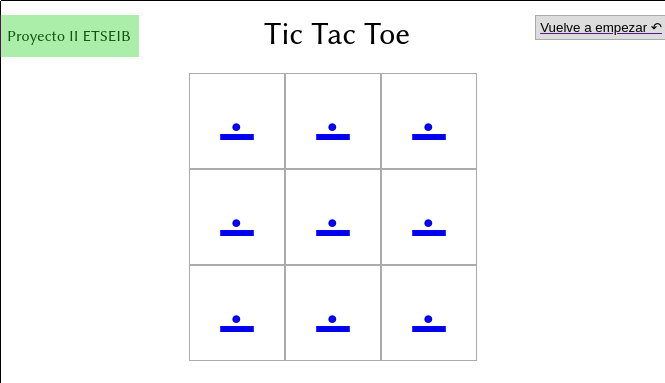
\includegraphics[width = .75\textwidth]{interfaz.png}}

    \caption{Interfaz Web}
  \end{figure}
  \note{
    LA IMAGEN ACTUA COMO UN LINK A TU WEB! (CLICAMOS en directo). \\
  }
\end{frame}


\begin{frame}{Movimiento brazo robótico}
  \begin{figure}
    \centering
    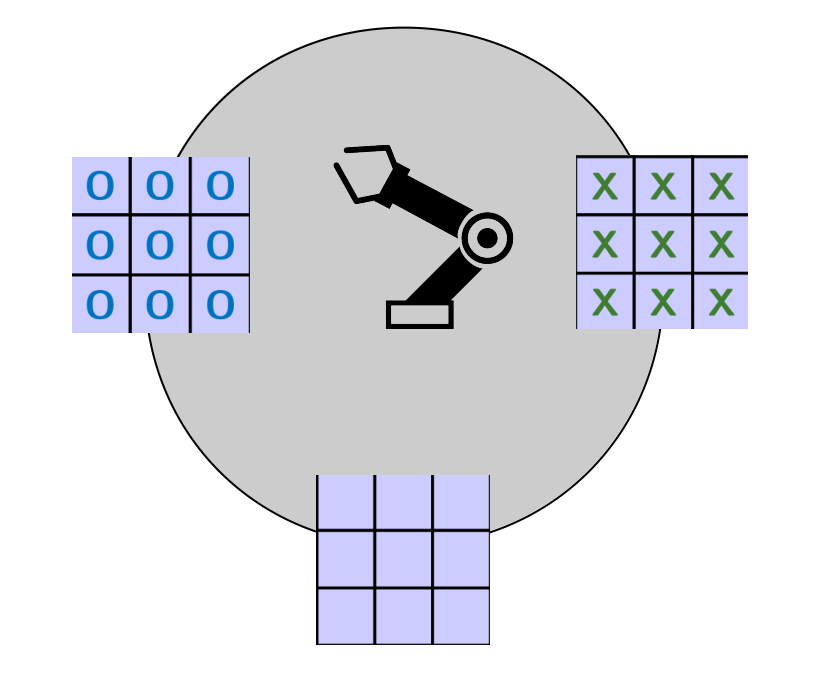
\includegraphics[width=6 cm]{Brazo_movimiento.png}
    \caption{Disposición circular del tablero}
  \end{figure}
\end{frame}

\begin{frame}{Movimiento brazo robótico II}
  \begin{columns}
    \column{0.6\textwidth}
    \begin{figure}
      \centering
      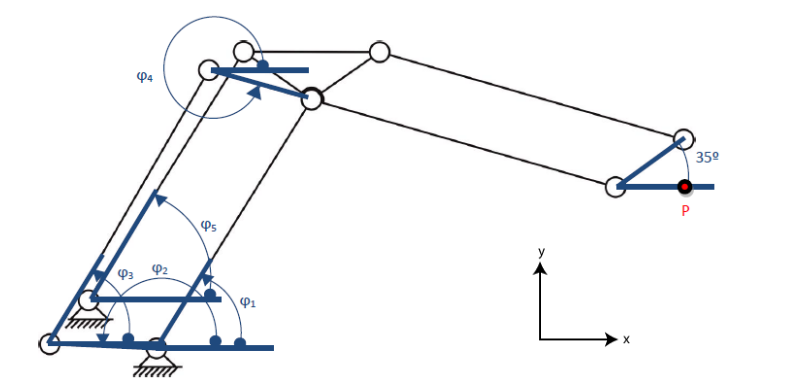
\includegraphics[width=4.9 cm]{Plano.png}
      \caption{Movimiento 2D}
      \label{fig:my_label}
    \end{figure}
    \begin{figure}
      \centering
      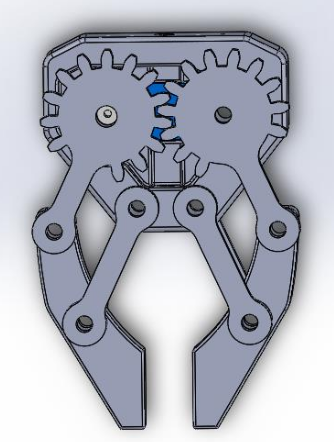
\includegraphics[width=2 cm]{Pinza.png}
    \end{figure}
    \column{0.4\textwidth}
    \textbf{Avances:}
    \begin{itemize}
      \item Script movimiento en un plano (Fallo servo)
    \end{itemize}

    \textbf{Por hacer:}
    \begin{itemize}
      \item Arreglar servo
      \item Control pinza y sincronización con el brazo
    \end{itemize}
  \end{columns}
\end{frame}

\end{document}